\documentclass[12pt]{article}

\usepackage[ngerman]{babel}
\usepackage[utf8]{inputenc}
\usepackage[scale=0.80]{geometry}
\usepackage{amsmath}
\usepackage{amssymb}
\usepackage{graphicx}
\usepackage{fancyhdr}
\usepackage{gensymb}

\renewcommand{\familydefault}{\sfdefault}
\renewcommand{\arraystretch}{1.25}
\setlength{\headheight}{28pt}
\pagestyle{fancy}

\lhead{\textbf{Datenbanksysteme II}\\
\textbf{Lösung von Aufgabe 3}}
\rhead{\textbf{Felix Wolff, Markus Petrykowski}\\
\textbf{Übungsgruppe B}}
\renewcommand{\footrulewidth}{0pt}

\begin{document}
\textbf{a)} Nach dem Einfügen der 1 ist das linke äußerste Blatt voll. Durch das
Einfügen der 4 muss es aufgeteilt werden in zwei Hälften. Die 3 aus dem neu
erstellten Knoten wird hochkopiert, sodass nun der linke innere Knoten voll
besetzt ist.

Beim Einfügen der 18 wird wieder nur das linksäußerste Blatt des rechten
Teilbaumes voll besetzt. Beim Einfügen der 20 muss dieses dann aufgeteilt,
und die 19 hochkopiert werden. Da der innere Knoten voll ist, wird dieser auch
geteilt in $[19,23]$ und $[31,41]$. Die 23 wird hochgeschoben. Die Wurzel ist
allerdings voll, sodass sie auch geteilt werden muss in $[17,23]$ und $[48,99]$.
Eine neue Wurzel mit Schlüssel 23 wird dann erstellt.

\begin{center}
    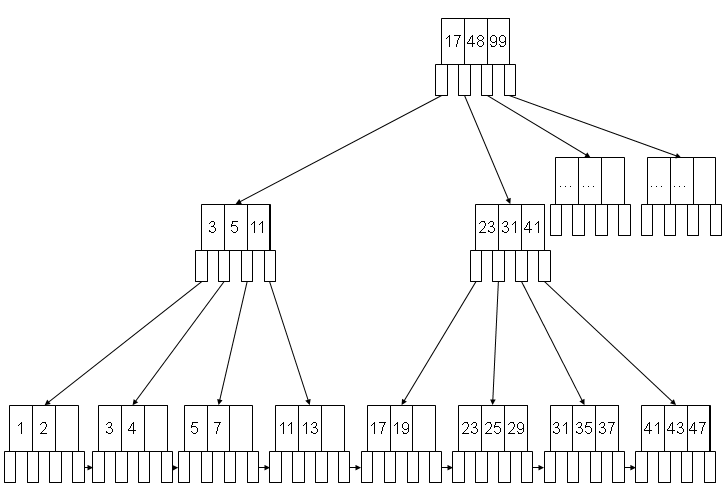
\includegraphics{insert_4.PNG}
    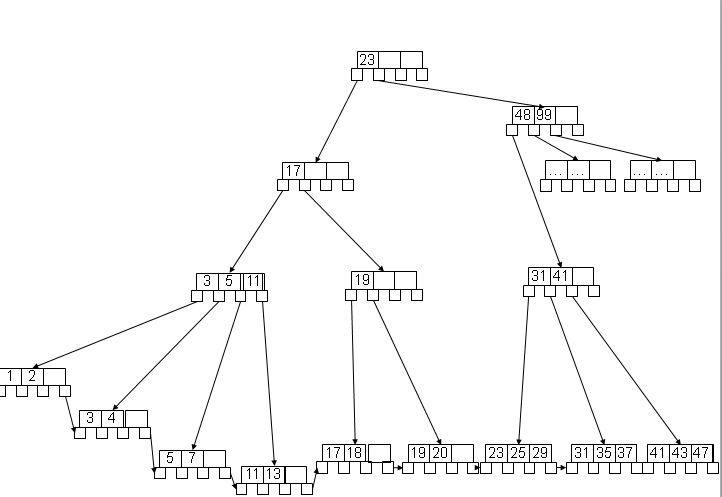
\includegraphics{insert_20.PNG}
\end{center}

\textbf{b)} Nach dem Entfernen der 1 ist der linke Knoten unterbesetzt und wird
mit dem rechten verschmolzen. Dadurch ist die Invariante, dass mindestens drei
Pointer verwendet sein müssen, wieder erfüllt. Der obere Knoten muss
dementsprechend auch die drei entfernt bekommen. Beim Löschen der 2 geschieht
nichts.

Beim Löschen der 3 muss wieder mit dem rechten Geschwisterknoten
fusioniert, und die 5 aus dem Vaterknoten entfernt werden, sodass dieser die
Invariante nun noch gerade so erfüllt. Beim Löschen der 4 passiert wieder
nichts.

Beim Löschen der 5 ist der Knoten der 7 unterbesetzt, und wird mit dem
rechten Geschwisterknoten fusioniert. Dadurch ist der innere Knoten unterbesetzt
und wird mit dem rechten Knoten verschmolzen. Dadurch ist wiederum dessen
Vaterknoten unterbesetzt. Dafür wird der Split-Key des Vaterknotens (der Wurzel)
runtergezogen, sodass nun die 23 im Knoten steht. Dann wird mit dem rechten
Geschwisterknoten fusioniert, sodass die nun leere Wurzel ersetzt wird.

Das Löschen der 7 ist dann wieder trivial - sie kann
einfach entfernt werden.
\begin{center}
    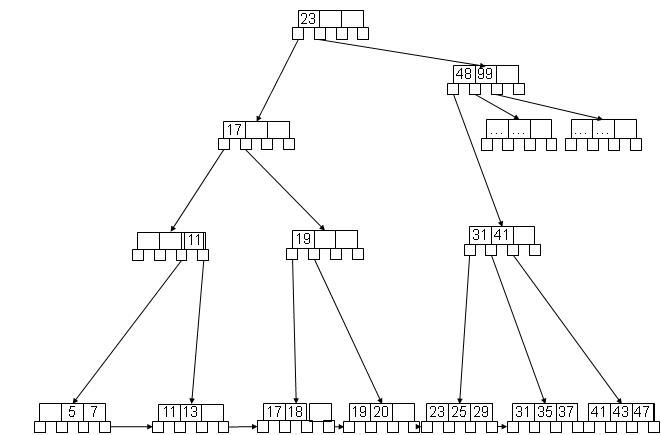
\includegraphics{delete_4.PNG}
    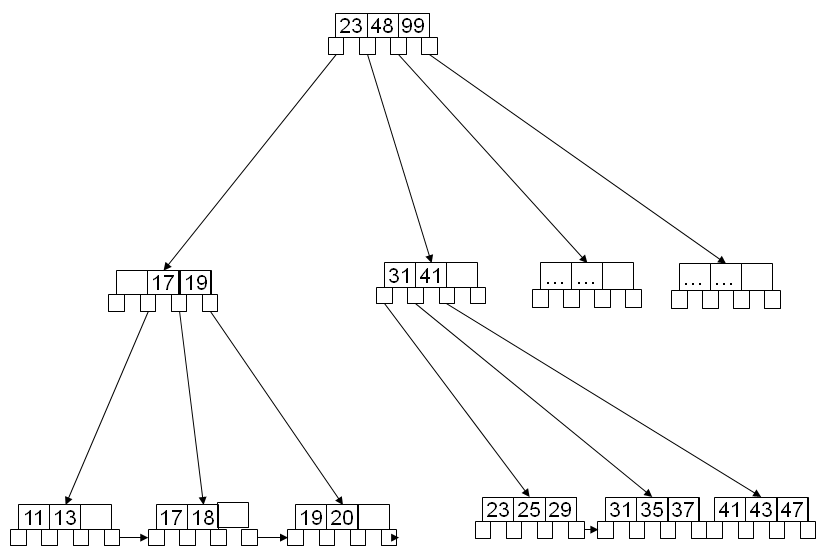
\includegraphics{delete_7.PNG}
\end{center}

\end{document}
% vim: tw=80
